\section{Human Motion Based Robot Motion Generation}
\label{sec:motion_generator}
In this research, we take human motions into account to decide robot motions with imitating them. According to the motion feature in each task, we sort the tasks in 3 classes -- manipulation i) by moving hands, ii) by walking, and iii) by holding with whole upper body -- and prepare the robot motion based on those human motion feature in each class. First, we describe the vision system used to acquire human motion information in \subsecref{vision}, and then the methods to decide the robot motions in each class in \subsecref{move_hand}, \subsecref{walk} and \subsecref{hold}.

\subsection{Visual Recognition to Acquire Human Motion Information}
\label{subsec:vision}
In order for robot to acquire human motion information, several approach can be considered. Using PointCloud measurements to get human skeleton, Microsoft Kinect or Xtion PRO Live can be applied. However, those techniques are limited to the detection of people whose bodies are not largely occluded by other objects. Since the robot needs to observe the human posture while manipulating large objects, these approaches won't be successful. To overcome that problem, we apply a visual recognition system using OpenPose~\cite{OpenPose}, which is the human detection technique using 2D images, to get the 3D positions of human limbs (\figref{detecting_limbs}). Since OpenPose has the characteristic in using a bottom-up method to detect human pose, it doesn't require the whole body to be seen.  In addition to it, HTC Vive system~\cite{vive} (\figref{vive}) is introduced to get the orientations of human limbs. HTC Vive system can measure the position and the orientation of each controller or tracker using infrared laser measurement. By attaching those devices on the human body, we can get the pose of each human limb (\figref{vive_on_body}).

\begin{figure}[htbp]
 \begin{center}
  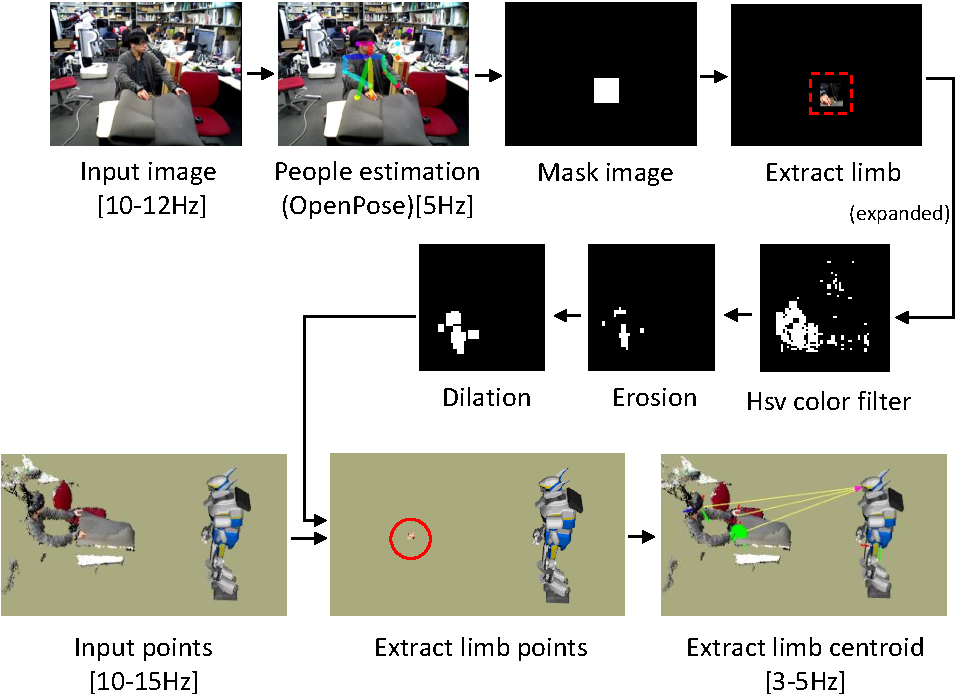
\includegraphics[width=1.00\columnwidth]{figs/openpose2}
  \caption{Getting the three dimensional positions of human hands and face during object manipulation.}
  \label{figure:detecting_limbs}
 \end{center}
\end{figure}

\begin{figure}[htbp]
  \begin{minipage}{0.45\hsize}
    \begin{center}
      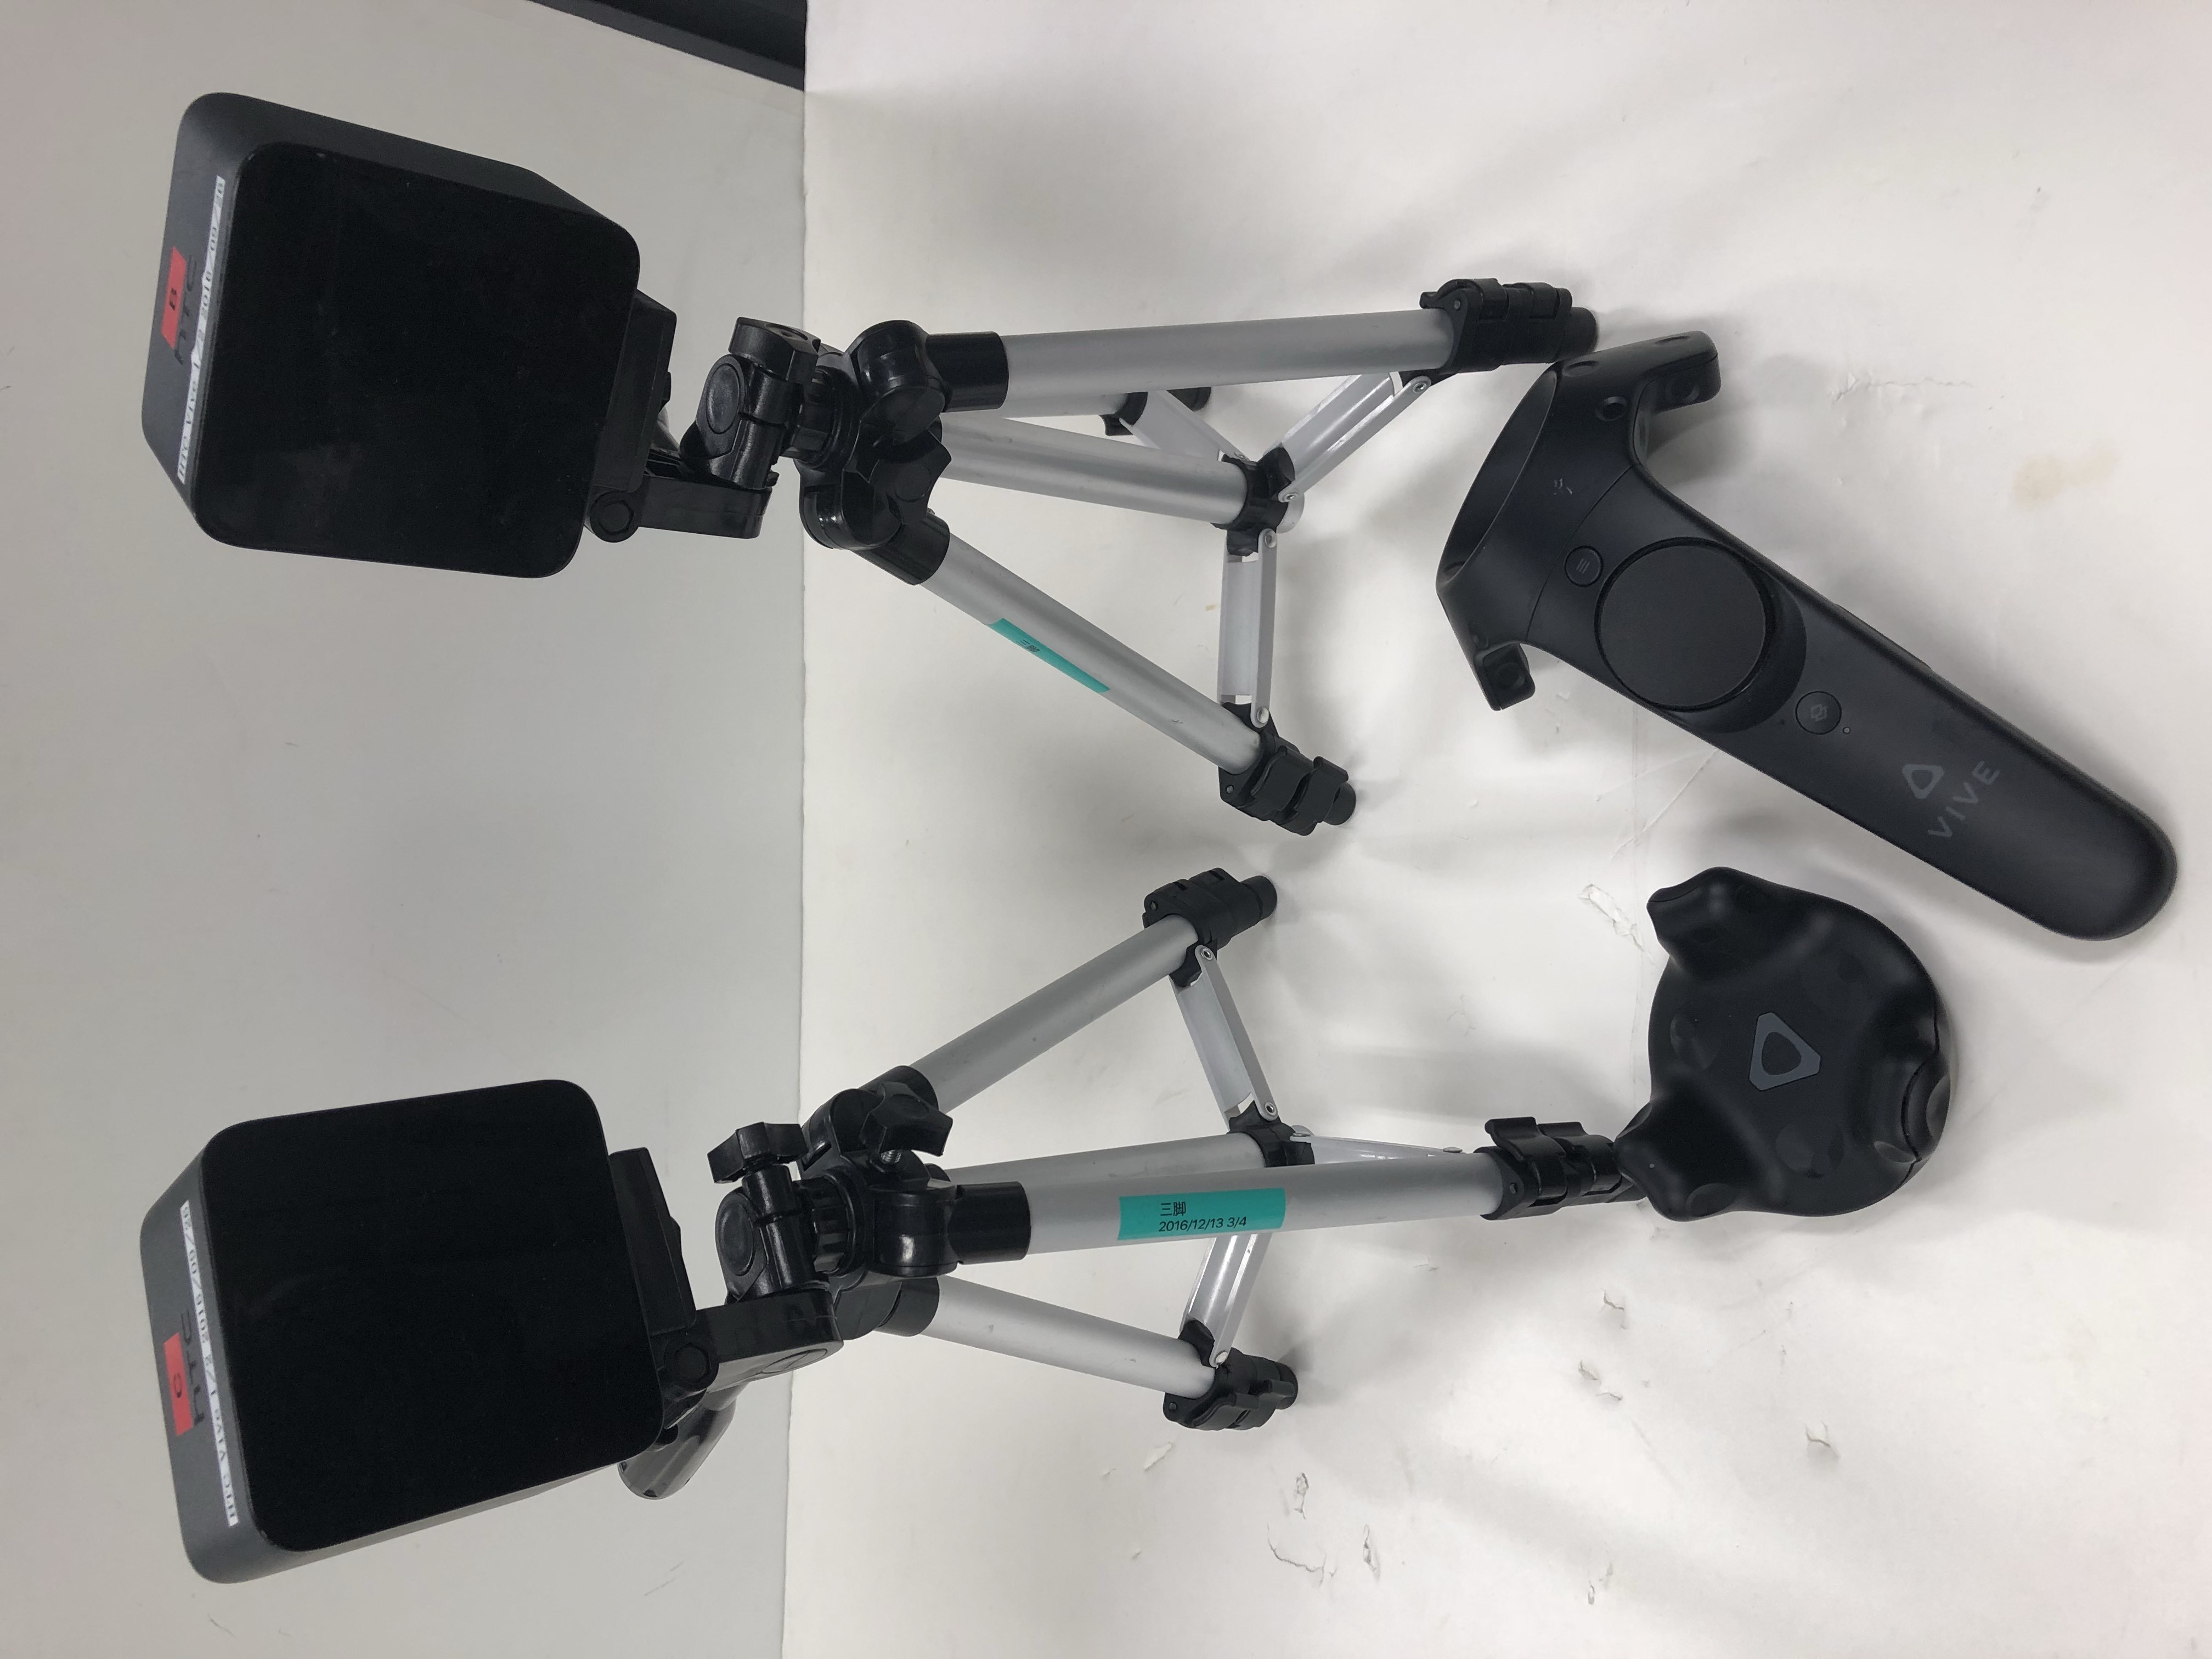
\includegraphics[angle=270, width=0.8\columnwidth]{figs/vive}
      \caption{HTC Vive system. A controller (right front) and a tracker (left front) recieve the IR laser from the two base stations called ``lighthouse'' and calculate the position and orientation.}
      \label{figure:vive}
    \end{center}
  \end{minipage}
  \begin{minipage}{0.45\hsize}
    \begin{center}
      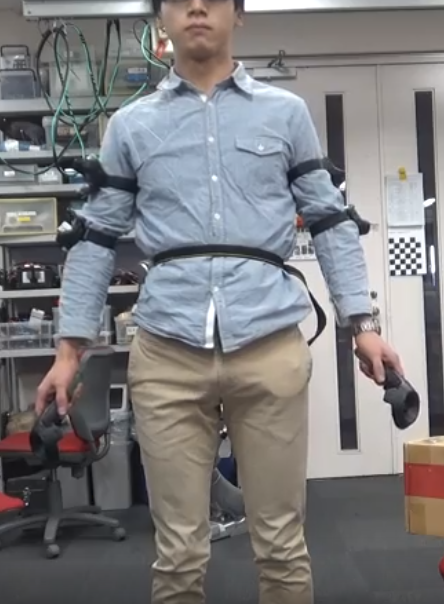
\includegraphics[width=0.8\columnwidth]{figs/vive_limb}
      \caption{The example of attaching the Vive trackers and the controllers on the human body.}
      \label{figure:vive_on_body}
    \end{center}
  \end{minipage}
\end{figure}

\subsection{Object Operation based on Hand Movement}
\label{subsec:move_hand}

\begin{figure}[htbp]
 \begin{center}
  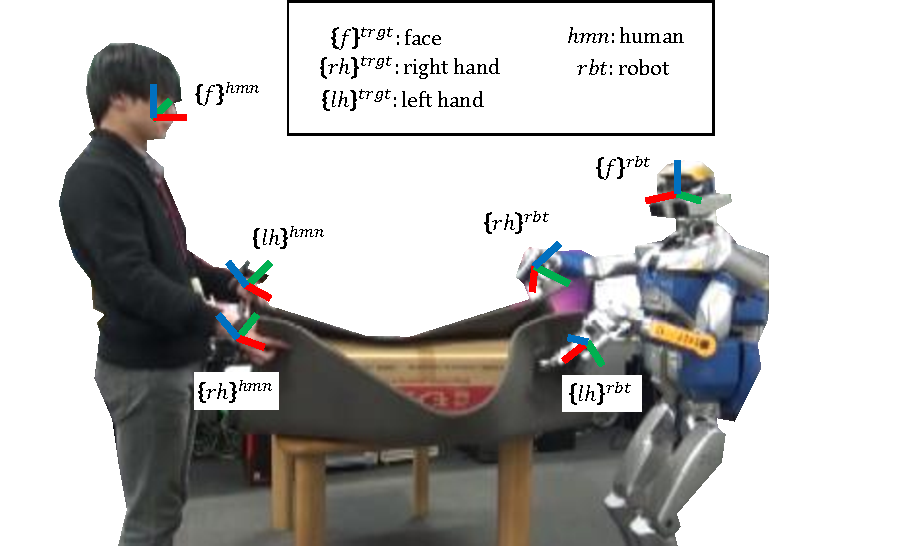
\includegraphics[width=1.00\columnwidth]{figs/coords_reference3}
  \caption{Coordinate reference used in this paper.}
  \label{figure:coords}
 \end{center}
\end{figure}

In situations of cooperative works where a human and a robot manipulate the same object at the same time with facing each other, we propose that the robot end effectors' coordinates can be decided by observing human hand motions and imitating them symmetry. \figref{coords} illustrates the reference frames and naming convention used in the rest of this paper. We focused on the hand coordinates \(\{rh\}\) and \(\{lh\}\) represented in the face coordinate \(\{f\}\). Using the homogeneous transformation matrixes \(\bm{T}^{trgt}_{h}\) and \(\bm{T}^{trgt}_{f}\), two coordinates of the hands \(\{rh\}\) and \(\{lh\}\) relative to the head coordinates \(\{f\}\) can be represented as homogeneous transformation matrixes \(^{f}\!\bm{T}^{trgt}_{h}\) as below.

\begin{align}
^{f}\!\bm{T}^{trgt}_{h} &= (\bm{T}^{trgt}_{f})^{-1}\bm{T}^{trgt}_{h}\\
{\rm where} \ \ trgt &\in \{rbt, hmn\},\nonumber \\
h &\in \{rh, lh\} \nonumber
\end{align}

%% \(^{f}\!\bm{T}^{trgt}_{h}\) can be converted into 6-dimentional vector \(^{f}\!\bm{t}^{trgt}_{h} = (\bm{p}^{\mathrm{T}} \; \bm{\phi}^{\mathrm{T}})^{\mathrm{T}} = (x \; y \; z \; \alpha \; \beta \; \gamma)^{\mathrm{T}}\).
A homogeneous transformation matrix \(\bm{T}\) can be converted into 6-dimensional vector \(\bm{t} = (\bm{p}^{\mathrm{T}} \; \bm{\phi}^{\mathrm{T}})^{\mathrm{T}} = (x \; y \; z \; \alpha \; \beta \; \gamma)^{\mathrm{T}}\). \(\bm{p} = (x \; y \; z)^{\mathrm{T}}\) represents the positions and \(\bm{\phi} = (\alpha \; \beta \; \gamma)^{\mathrm{T}}\) represents the Euler angles in the ZYX convention. Considering two coordinates of the human hands, the desired robot end effectors' positions and orientations are determined as below. %% Considering two coordinates of the hands, the desired end effectors' positions are determined as below.

\begin{align}
  %% ^{f}\!\bm{p}^{rbt}_{h} &=
  %% \left(
  %% \begin{array}{rrr}
  %%   1 & 0 & 0 \\
  %%   0 & -1 & 0 \\
  %%   0 & 0 & 1
  %% \end{array}
  %% \right) \;
  %% ^{f}\!\bm{p}^{hum}_{h'}\\
  %% ^{f}\!\bm{\phi}^{rbt}_{h} &=
  %% \left(
  %% \begin{array}{rrr}
  %%   -1 & 0 & 0 \\
  %%   0 & 1 & 0 \\
  %%   0 & 0 & -1
  %% \end{array}
  %% \right) \;
  %% ^{f}\!\bm{\phi}^{hum}_{h'}\\
  \left(
  \begin{array}{r}
    ^{f}\!x^{rbt}_{h}\\
    ^{f}\!y^{rbt}_{h}\\
    ^{f}\!z^{rbt}_{h}\\
  \end{array}
  \right)
  &=
  \left(
  \begin{array}{r}
    ^{f}\!x^{hmn}_{h'}\\
    -^{f}\!y^{hmn}_{h'}\\
    ^{f}\!z^{hmn}_{h'}\\
  \end{array}
  \right),\\
  \left(
  \begin{array}{r}
    ^{f}\!\alpha^{rbt}_{h}\\
    ^{f}\!\beta^{rbt}_{h}\\
    ^{f}\!\gamma^{rbt}_{h}\\
  \end{array}
  \right)
  &=
  \left(
  \begin{array}{r}
    -^{f}\!\alpha^{hmn}_{h'}\\
    ^{f}\!\beta^{hmn}_{h'}\\
    -^{f}\!\gamma^{hmn}_{h'}\\
  \end{array}
  \right)\\
  {\rm where} \ \ h \cup h' &= \{rh, lh\} \nonumber
  %% \label{equation:desired_hand_pos}
\end{align}

\begin{figure*}[htbp]
 \begin{center}
  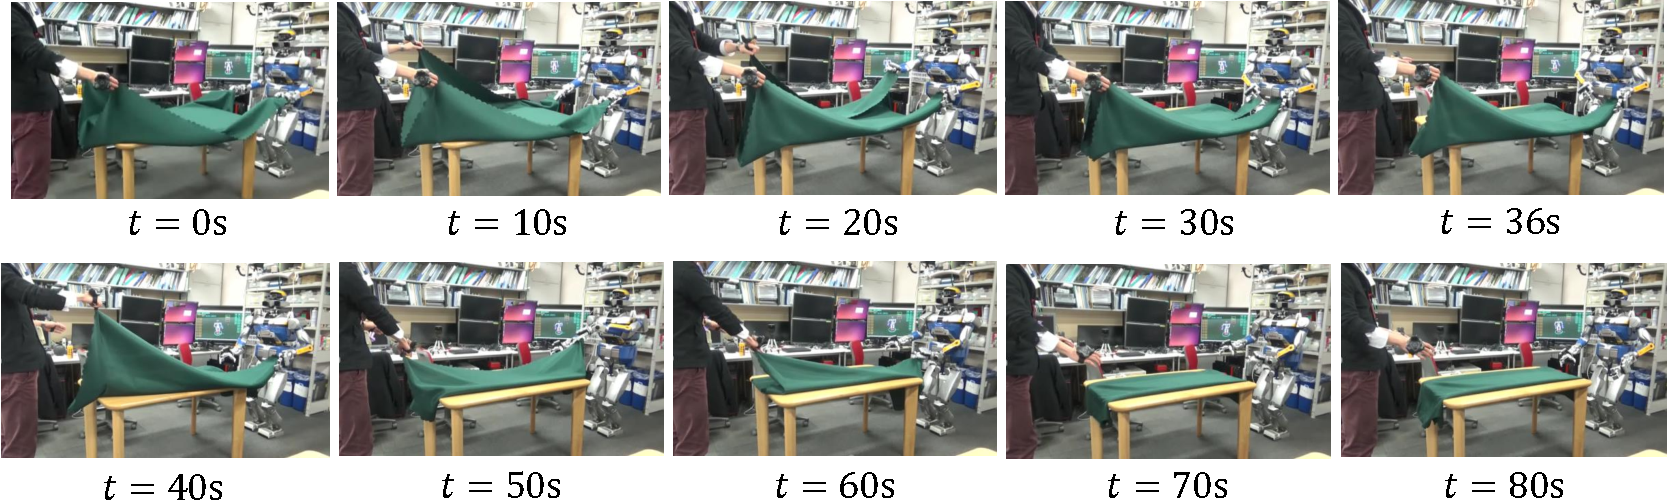
\includegraphics[width=2.00\columnwidth]{figs/cloth_folding}
  \caption{The experiment of folding a large cloth by a human and a robot. At \(t=\SI{36}{s}\) and \(t=\SI{60}{s}\), the human make the robot release its hand by using voice instruction.}
  \label{figure:folding_cloth}
 \end{center}
\end{figure*}

Here, to decide robot right hand target coordinates, those of human left hand are used. The same can be said for the reversed.
%
%% \begin{align}
%% \bm{T}^{rbt}_{h} &= \bm{T}^{rbt}_{f} {}^{f}\!\bm{T}^{rbt}_{h}\\
%% {\rm where} \ \ h &\in \{rh, lh\} \nonumber
%% \end{align}

We solve Inverse Kinematics (IK) with these end effectors' constraints and get the robot angle vector. When time series angle vectors are applied to the real robot, there are three major constraints or difficulties, described in \cite{adapt_human_motion}.
\begin{enumerate}
  \item joint angle limits
  \item joint angular velocity limits
  \item motion around the gimbal lock
\end{enumerate}
In the previous researches, human motions of actors or dancers are applied to those of robot~\cite{adapt_human_motion}\cite{bandaisan} with satisfying these restrictions with various optimizations. However, since these approaches are executed offline, these methods are not so useful here where online movement is required and not so much about the exact timing. Therefore, in this research, we take temporal solutions; limiting the area where the robot can move its hands in order not to violate \(1)\) and \(3)\), and setting the interpolating time on the real robot joint angles as \SI{4}{sec} so that \(2)\) can be eased.\par

\figref{folding_cloth} shows a short experiment proving that these robot motions work suitably in the task of folding a table cloth by a human and a robot grasping each side of it. At \(t=\SI{36}{s}\) and \(t=\SI{60}{s}\), using also the aural instructions, the human order the robot to release its right or left hand.\par

\subsection{Cooperative Carrying Following Human Walking}
\label{subsec:walk}
In case that transportation of the object are needed for executing the task, we also introduced a robot walking motion by observing human velocity and position. In the previous researches, the walking direction or the speed of the robot is controlled by the interactive force or torque~\cite{aist_cooperative_carrying}\cite{carry_table}. Although rigid objects can be carried using those methods, they cannot be applied to carry flexible objects like cloth. To overcome that problem, we introduced a method to generate robot velocity considering human velocity and position as below.

\begin{align}
v^{rbt}_{vel, t+1} &= v^{rbt}_{vel, t} + f_{vel}(v^{hmn}_t) \label{equation:v_vel}\\
v^{rbt}_{pos, t} &= f_{pos}(x^{hmn}_t-x^{hmn}_{d}) \label{equation:v_pos}\\
v^{rbt}_{real, t} &= v^{rbt}_{vel,t} + v^{rbt}_{pos,t} \label{equation:v_real}\\
{\rm where} \ \ v^{hmn}_{t} &= \frac{x^{hum}_{t} - x^{hum}_{t-\Delta t}}{\Delta t} \nonumber
\end{align}

\(v^{rbt}_{vel, t}\) represents the robot velocity considering the human velocity \(v^{hmn}_{t}\), and \(v^{rbt}_{pos, t}\) represents the robot velocity considering the human position \(x^{hmn}_{t}\) compared with the desire position \(x^{hmn}_{d}\). Note that \(v^{hmn}_{t}\) and \(x^{hmn}_{t}\) are the velocity and the position relative to that of the robot, and not the absolute value. Finally, \(v^{rbt}_{real, t}\) represents the robot velocity applied to the real robot. The function \(f\) is described as below and the graph of it is shown in the left in \figref{func_f}.
\begin{equation}
  \begin{footnotesize}
  f(x) =
  \begin{cases}
    -v_{max} & (x < -thre - \frac{v_{max}}{gain}) \\
    gain\cdot(x+thre) & (-thre - \frac{v_{max}}{gain} \le x < -thre) \\
    0 & (-thre \le x < thre) \\
    gain\cdot(x-thre) & (thre \le x < thre + \frac{v_{max}}{gain}) \\
    v_{max} & (otherwise) \\
  \end{cases}
  \end{footnotesize}
\end{equation}

\equref{v_vel}-\equref{v_real} can be simplified to the equation below.
\begin{align}
%% \Delta v^{rbt} &= K_p(v^{hmn}_{abs} - v^{rbt}) + K_i\int (v^{hmn}_{abs} - v^{rbt}) dt
\Delta v^{rbt} &= v^{rbt}_{real, t+1} - v^{rbt}_{real, t}\\
&= K_p(v^{hmn}_{abs} - v^{rbt}) + K_i\sum (v^{hmn}_{abs} - v^{rbt}) \Delta t
\end{align}
This can be recognized as a PI controller to let the robot velocity match the human velocity giving proper parameters \(K_p\) and \(K_i\), which correspond to the parameter \(gain\) in the function \(f\).

\begin{figure}[htbp]
  \begin{center}
    \begin{minipage}{0.45\hsize}
      \begin{center}
      %% 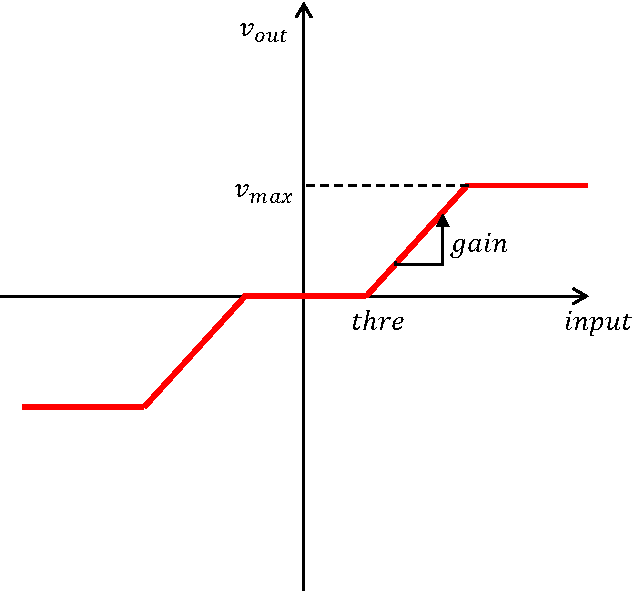
\includegraphics[width=1.00\columnwidth]{figs/func_f}
      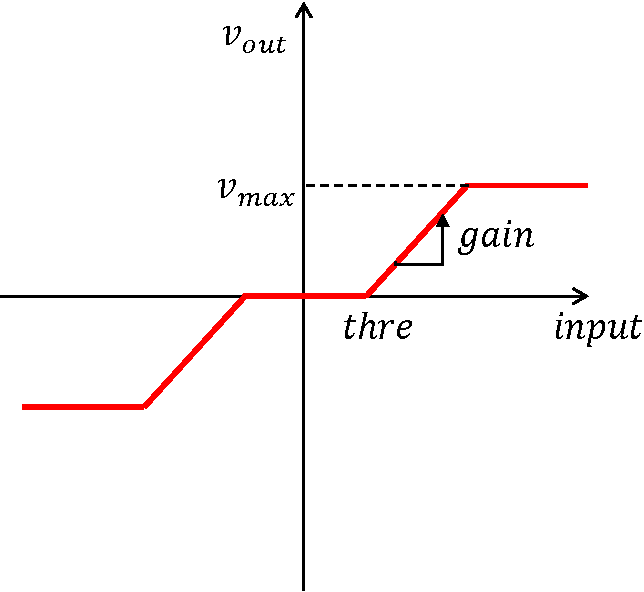
\includegraphics[width=1.00\columnwidth]{figs/filter_vel_1}
      \end{center}
    \end{minipage}
    \begin{minipage}{0.45\hsize}
      \begin{center}
        %% 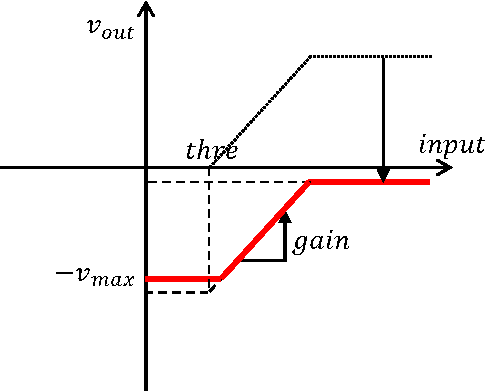
\includegraphics[width=1.00\columnwidth]{figs/func_f_}
        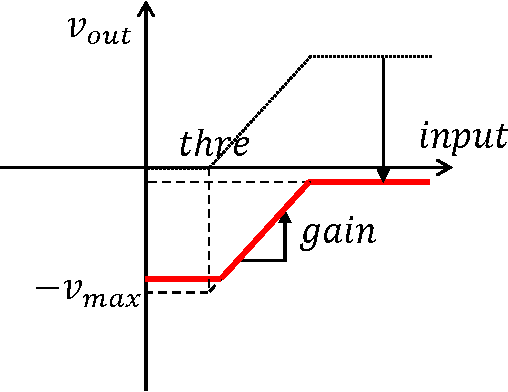
\includegraphics[width=1.00\columnwidth]{figs/filter_vel_2}
      \end{center}
    \end{minipage}
    \caption{The left represents a graph of a filter to generate robot velocity from human velocity or human position. Constant \(thre\), \(gain\) and \(v_{max}\) are the given parameters according to the walking direction. The right represents a graph of a filter to generate robot velocity from human position when the human and the robot are moving in the opposite direction back.}
    \label{figure:func_f}
  \end{center}
\end{figure}

On the other hand, there will be a situation that the two operators move in the opposite direction close or away when manipulating flexible objects; folding clothes with approaching each other or stretching them with taking a distance between each other. In such situation, velocity is not so much important than moving in the same direction with carrying the same thing. We consider only position when the two moving against each other.
\begin{align}
v^{rbt}_{t} &= v^{rbt}_{pos,t} = f_{pos}(x^{hmn}_t)
\end{align}
The same function \(f\) can be applied when the two move in the opposite direction close. The right in \figref{func_f} shows a new graph applied when the two move in the opposite direction away.\par

To secure the use with rigid objects, we take haptic information into account in the feedback layer. Using the methods above, the robot can recognize when to stop by observing human velocity and position. However, in order to carry rigid large objects by the two, this may not sometimes be enough. Because of the relatively low frequency of the visual recognition, the robot may not be able to respond to the sudden stop of the counterpart. This causes an unexpected falling down of the robot. Preventing this accident, we introduce the feedback layer that the robot stops walking when feeling unexpected force against the walking direction. This can be used not only to prevent the accident, but also to suggest that it's an enough distance to take, when, for example, the two are grabbing each side of the cloth and stretching it.

Finally, the aural instruction of the direction by the human is combined. Which direction to move can be decided by the human and announcing it, robot can start moving with the velocity generation explained above.

\subsection{Passing Large Objects based on Arm Posture}
\label{subsec:hold}
In order to carry large objects, we need to use whole upper body including arms. When passing those objects from a human to a robot, the robot can watch how the human holds them and regard those postures as suitable ones to hold the objects whose weight is unknown. We get the positions and orientations of human 7 points (shoulders, elbows, hands and torso) to reconstruct the human posture carrying the object, and apply them to the robot to make the similar posture to the human. However, passing objects cannot be succeeded only by it. We take a mean of fixing robot posture by human teaching in order for the robot to hold the objects stably.\par
To acquire the robot angle vector, two methods can be considered; IK based approach and joint-space based approach. The former approach ensures the end effector be fixed to the target coordinate. It is useful when executing tasks where the position and orientation are important; reaching and picking a certain object. However, to hold large objects, the whole posture of arms appears to be more essential than exact position or orientation. Although those arm postures might be able to be generated with adding other constraints when calculating IK, it causes more failure in IK solution. Therefore, we take the joint-space approach considering each direction of human limb where the above weaknesses in IK don't appear.\par
Using the Vive system, position and orientation information of human shoulders, elbows, hands and the torso are gotten. We apply those information to the robot to consider the robot arm posture. %% Note that body concealed by the holding object.
The robot has 7 DoF in its each arm; 3 DoF in shoulder, 1 DoF in elbow, 3 DoF in wrist. The angles of these joints are calculated as below.
\begin{enumerate}
 \item The roll and pitch joint angle of shoulder are calculated by desired shoulder direction \(^{sh}\!\bm{v}^{hmn}_{el}\).
 \item The pitch joint angle of elbow are calculated by the angle between \(^{sh}\!\bm{v}^{hmn}_{el}\) and \(^{el}\!\bm{v}^{hmn}_{hnd}\).
 \item The yaw joint angle of shoulder is calculated by the angle between \(\bm{n}^{hmn}\) and \(\bm{n}^{rbt}\) that are the normal vectors of the planes that contain \(^{sh}\!\bm{v}^{trgt}_{el}\) and \(^{el}\!\bm{v}^{trgt}_{hnd}\).
 \item The roll, pitch and yaw joint angle of wrist are calculated by solving IK with only 3 DoF in the wrist.
\end{enumerate}

Vectors used above are illustrated in \figref{arm_posture}.

\begin{figure}[htbp]
 \begin{center}
  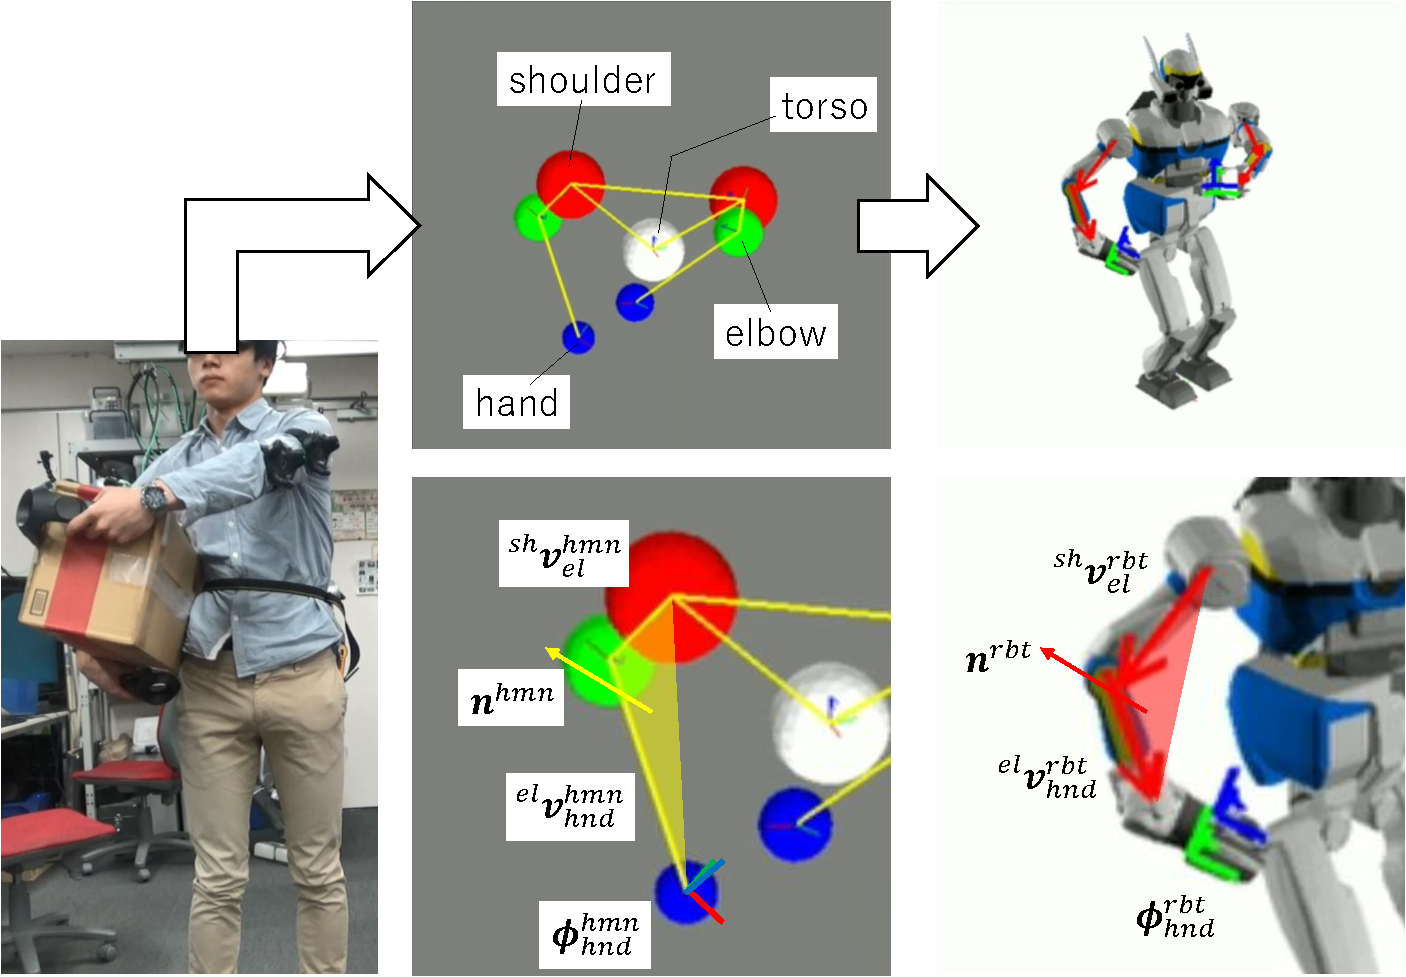
\includegraphics[width=1.00\columnwidth]{figs/arm_posture2}
  \caption{Arm posture generation in robot.}
  \label{figure:arm_posture}
 \end{center}
\end{figure}

Taking the average of the time series robot upper-body postures calculated with the above calculation, we decide one pre-grasp robot posture and apply to the real robot, supposing the human postures when holding an large object are almost unchanged.

Holding large objects cannot be realized only by the above process. Although the robot links are configured similar to those of human, each link length of the robot is not exactly the same as human. Moreover, to hold objects, pre-grasp poses leading the final grasping poses are needed~\cite{pregrasp}. To satisfy those requirements, we settle this problem by introducing physical interaction. As noted above, the posture of the upper body is important to hold large objects. To preserve the posture made through the above process, a system is introduced where a human can move each joint by choosing which joint to move by voice and the extent of the change in the joint angle is determined according to the extent of force.\par
\figref{passing} shows the snapshots of the experiments passing large boxes from a human to a robot. First, the robot takes an pose acquired by considering human holding pose. Here, it has to be noted that the posture the robot takes are right/left inverted as that of human. Then, with human fixing the robot posture by force and voice, the human-robot object passing is executed, finally the robot stepping in the position with holding the boxes.

\begin{figure*}[htbp]
 \begin{center}
  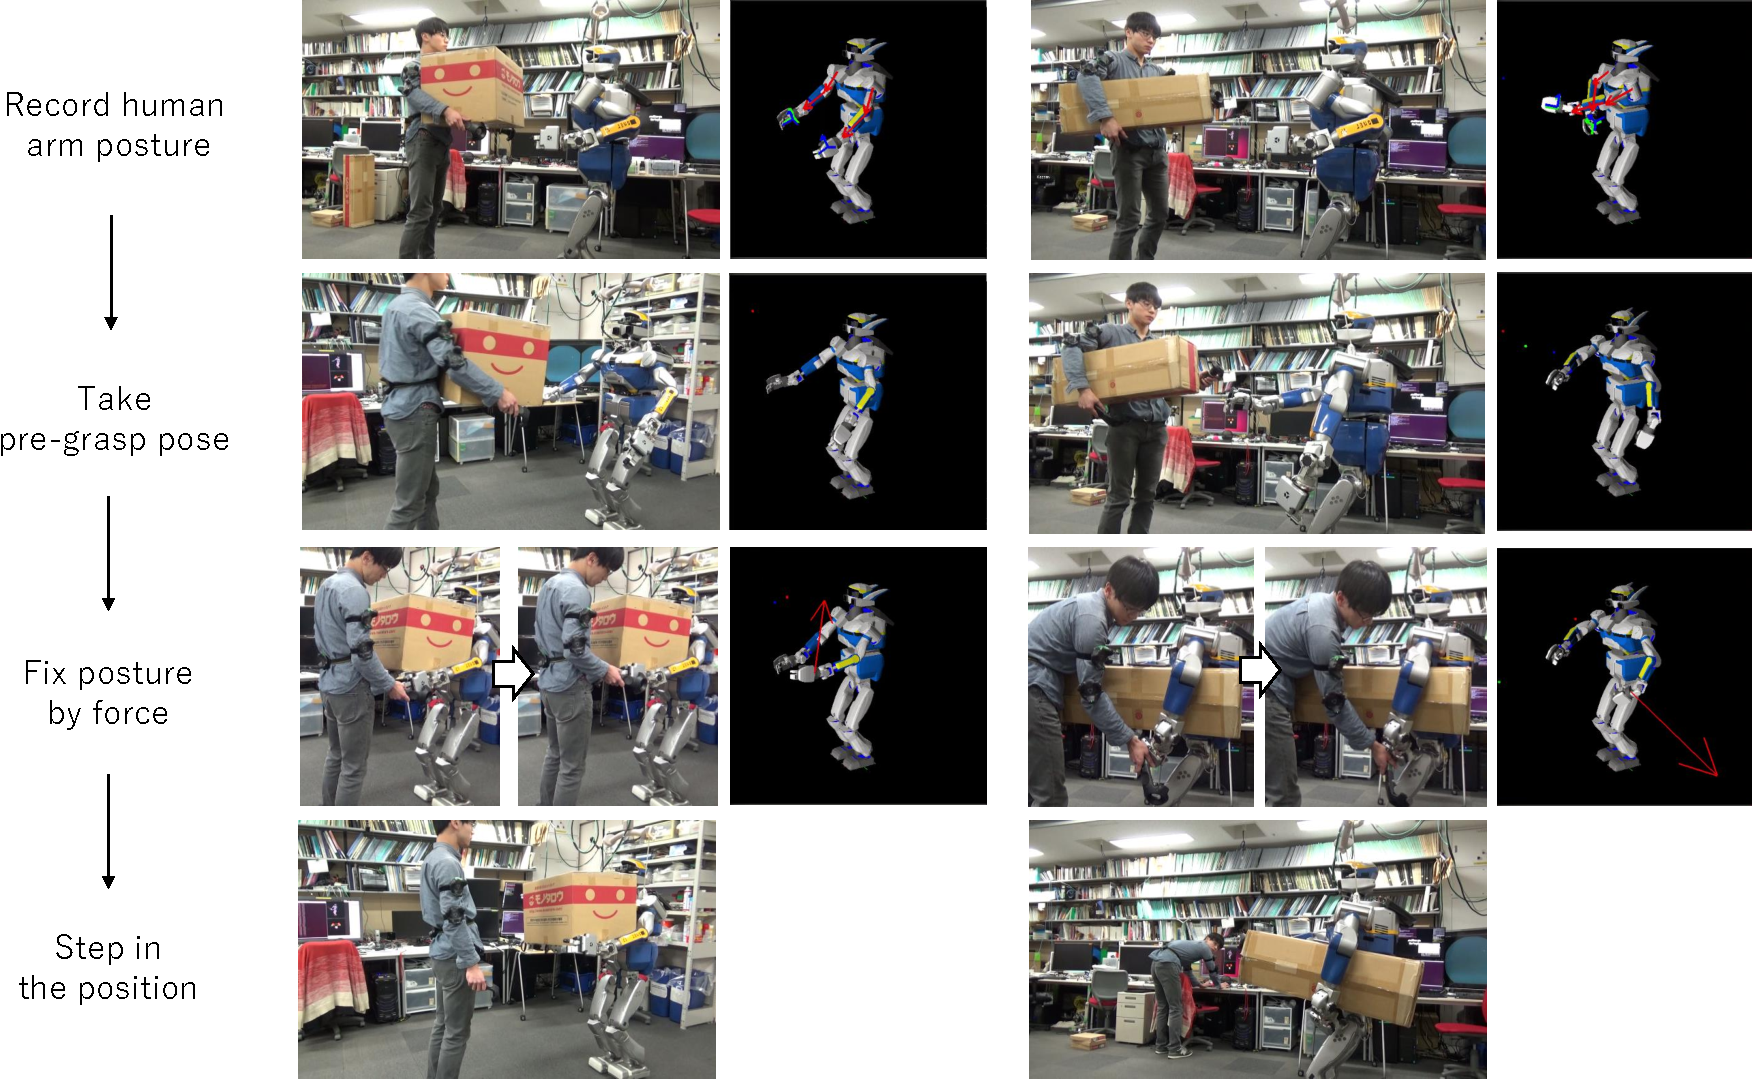
\includegraphics[width=2.00\columnwidth]{figs/passing_ex2}
  \caption{The experiments of passing objects from the human to the robot.}
  \label{figure:passing}
 \end{center}
\end{figure*}

%% \begin{figure}[htbp]
%%  \begin{center}
%%   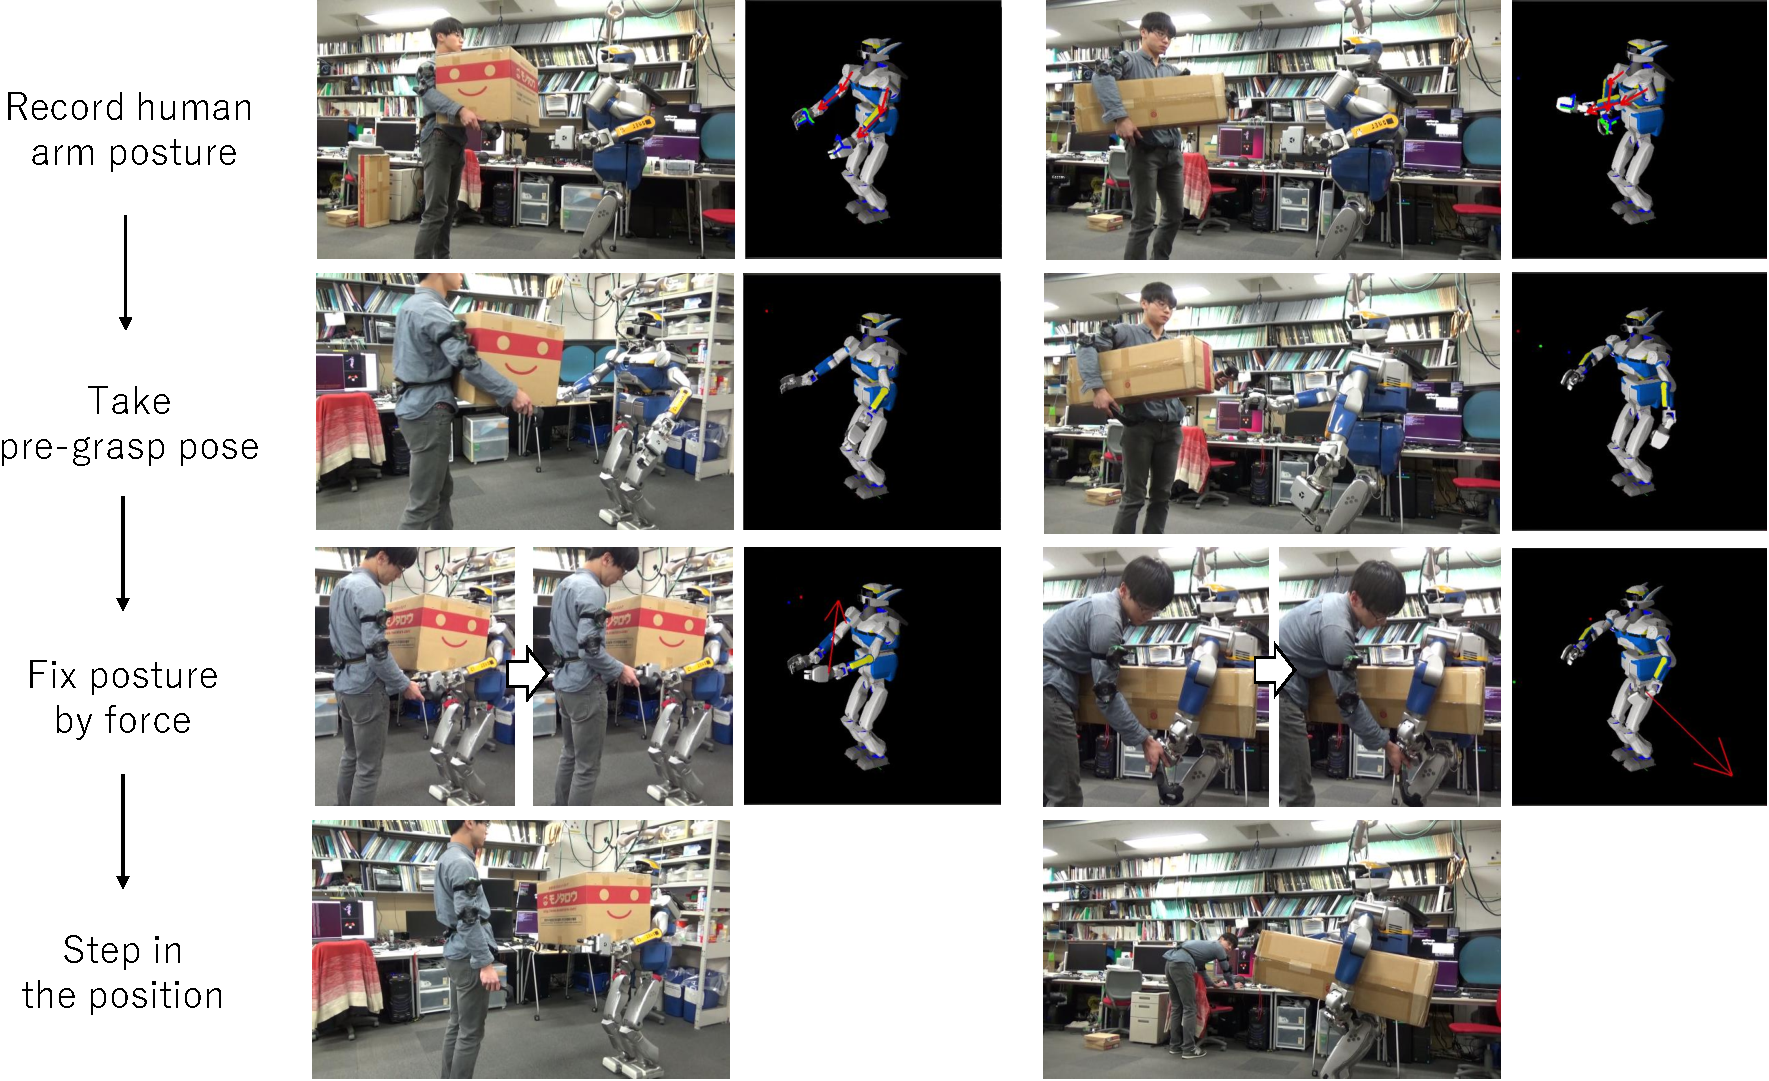
\includegraphics[width=1.00\columnwidth]{figs/passing_ex}
%%   \caption{The experiments of passing objects from the human to the robot.}
%%   \label{figure:passing}
%%  \end{center}
%% \end{figure}
